\documentclass{article}
\usepackage{amsmath}
\usepackage{graphicx}
\usepackage{hyperref}
\title{PhysLang: A Domain Specific Language for Physical Simulation using Generalized Coordinates}
\author{Desai Chen, David I.W. Levin, Shinjiro Sueda, Wojciech Matusik}
\begin{document}
\maketitle

\section{Design Goals}

\section{Describing Physical Objects}
TODO: Add mapping-element description and diagram here.

\section{Analysis of Time Stepper}

An example: Below are the Function Graph and Time Line for the velocity update step of the Forward Euler Integrator for a single particle. The goal of this stage of the integrator is to compute

\begin{equation}
\mathbf{q}^{t+1} = \mathbf{q}^t + \Delta t \mathbf{M}^{-1}\mathbf{f}\left(t\right). 
\end{equation}  Here we distinguish the discrete $t$ variable used here from the continuous time used above.  

We can express the functional relationships  in this equation as a simple graph where ellipses are functions and arrows indicate the flow of information between functions (\autoref{fig:funcgraph}). As yet all of our functions of undefined input and output data types as these can only be divined now that the time stepper is known.

\begin{figure}[h]
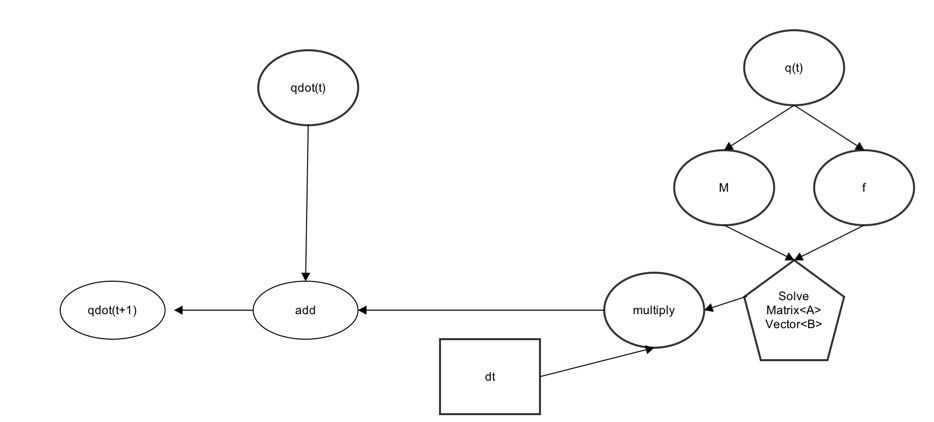
\includegraphics[width=0.9\textwidth]{figures/functiongraph}
\caption{Function Graph: Data flow between abstract functions shown as ellipses. }
\label{fig:funcgraph}
\end{figure}

We will proceed in the following stages, which will be detailed below
\begin{itemize}
\item Configuration Variable Substitution
\item Edge Removal
\item Data Type Propagation
\item Concrete Function Instantiation
\end{itemize}

\subsection{Configuration Variable Substitution}
The first step of our process to analyze how many time states we need to store for $\mathbf{q}$ and $\dot{\mathbf{q}}$. In this example it is easy to see that we require storage for $\mathbf{q}^t$, $\dot{\mathbf{q}^{t+1}}$ and $\dot{\mathbf{q}^{t}}$. We replace these with typeless variables shown as squares in our graph (\autoref{fig:qt}).

\begin{figure}[h]
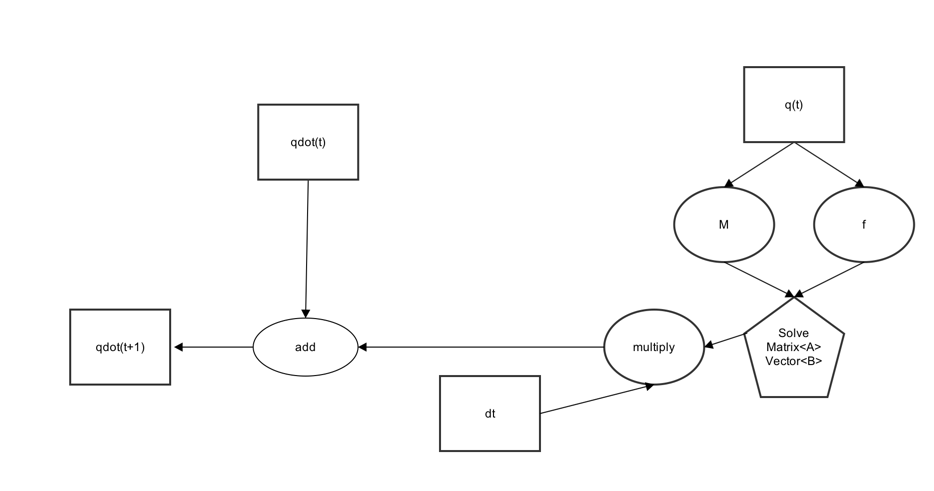
\includegraphics[width=0.9\textwidth]{figures/qtsubstitution}
\caption{Configuration functions are replaced  }
\label{fig:qt}
\end{figure}

\subsection{Data Type Propagation}
Our goal will be to assign types to each edge of the graph. These types then correspond to the concrete data types that should be taken as input by and given as output from each function. Once every edge incident on a function has an assigned type we can transform this abstract function (ellipse) into a concrete function shown by a hexagon which contains the specific types used. Note that in our simple example we begin with one concrete function, our linear solver, which requires a specific matrix and vector type as input and a specific vector type as output. We proceed by propagating these types through the function graph in a breadth first manner using a set of simple proportion rules (\autoref{fig:propagate}).

\begin{figure}[ht]
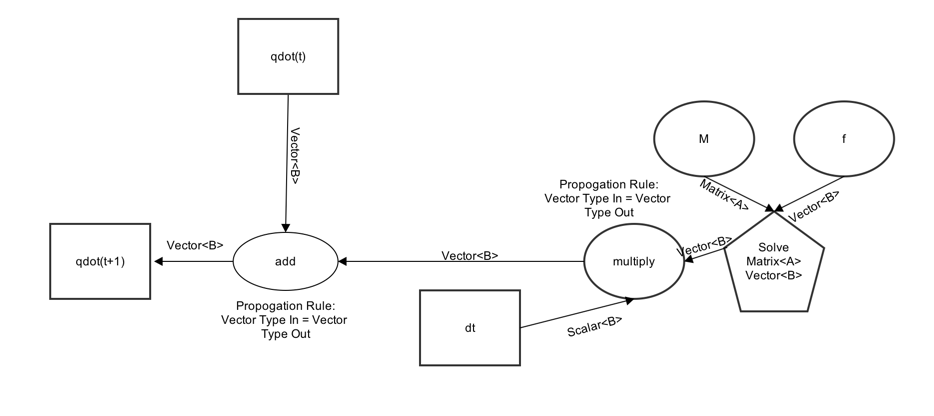
\includegraphics[width=0.9\textwidth]{figures/propagateTypes}
\caption{Type propagation and simple rules  }
\label{fig:propagate}
\end{figure}

\subsection{Instantiate Concrete Functions}
Once all edges have been assigned variable types we can instantiate concrete functions using these types for input and output parameters. In this case we have no conflicting assignments  (edges with more than one type label) and so we can trivially build these functions. More complicated cases will require additional rules to resolve them (\autoref{fig:concrete}).

\begin{figure}[ht]
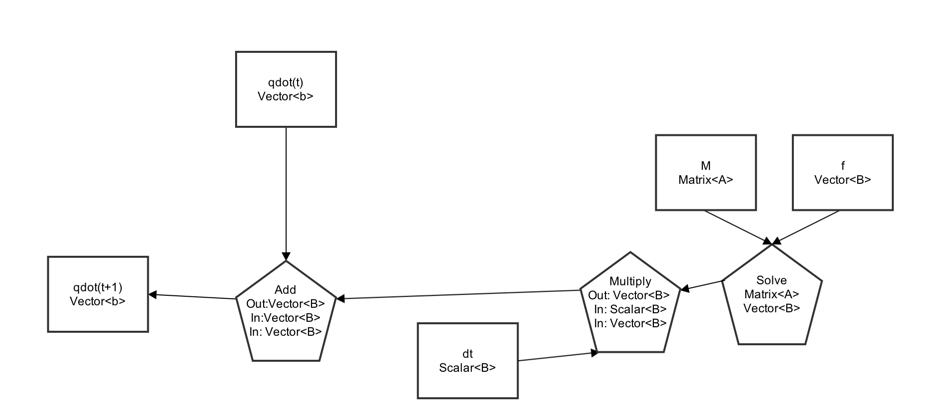
\includegraphics[width=0.9\textwidth]{figures/instantiategraph}
\caption{The graph of concrete functions, shown as hexahedral nodes.  }
\label{fig:concrete}
\end{figure}


\end{document}

